%% ------------------------------------------------------------------------- %%
\chapter{Algoritmos}
\label{cap:algoritmos}

Este cap�tulo descreve o processo de escolha e desenvolvimento dos algoritmos usados na elabora��o deste trabalho. Ambos foram desenvolvidos em linguagem C, sem o uso de bibliotecas externas, e sob as restri��es impostas pelo arcabou�o LegUp referente �s t�cnicas e recursos da linguagem que poderiam ser utilizadas no fluxo de puro \textit{hardware}.

Tal fluxo foi utilizado devido � mudan�a radical entre um algoritmo programado para um processador comum, e o mesmo algoritmo rodando puramente em \textit{hardware}. Usar os fluxos h�brido ou de puro \textit{software} trariam muitas semelhan�as a sistemas j� existentes e, possivelmente, mais eficientes, como sistemas embarcados com uso de microprocessadores (e.g. placas Arduino) ou mesmo um computador pessoal de prop�sito geral.

\section{Compress�o de dados}

Nos tempos atuais, uma quantidade massiva de dados � produzida diariamente. Por exemplo, estima-se que a rede social Twitter, no segundo quadrimestre de $2018$, possuiu uma m�dia de $335$ milh�es de usu�rios ativos mensais (https://investor.twitterinc.com/static-files/4bfbf376-fefd-43cc-901e-aedd6a7f1daf). Se cada usu�rio publicar um texto de $140$ caracteres ASCII, que possuem $1$ \textit{byte} cada, ser�o gerados $46,9$ \textit{gigabytes} em um �nico instante. Apesar de parecer uma quantia baixa, a hip�tese � de que cada usu�rio publique apenas uma vez no m�s, o que � irrealista. Dessa forma, podemos supor que essa rede social, sozinha, produz mensalmente uma quantidade de dados v�rias ordens de grandeza maiores que isso. Na verdade, estima-se que os servidores do Twitter armazenem cerca de $250$ milh�es de publica��es por dia (REFERENCIAS AQUI: https://www.quora.com/How-much-data-does-Twitter-store-daily).
	
Essa quantidade de dados pode ser utilizada para aplica��es modernas, como an�lise de sentimentos ou aprendizado de m�quina. Ainda assim, � necess�rio uma forma eficiente de armazen�-la e transport�-la. Nesse contexto, surgem os algoritmos de compress�o de dados, muito utilizados por \textit{softwares} de compress�o de arquivos e por bancos de dados. Dentre tais algoritmos, um � relativamente simples e eficiente para grandes sequ�ncias de dados: o algoritmo de Huffman.

\subsection{Algoritmo de Huffman}

\subsection{Implementa��o}

\section{Aproxima��o do problema do caixeiro viajante}



Um exemplo de figura est� na figura~\ref{fig:graph}.
\begin{figure}[htb]
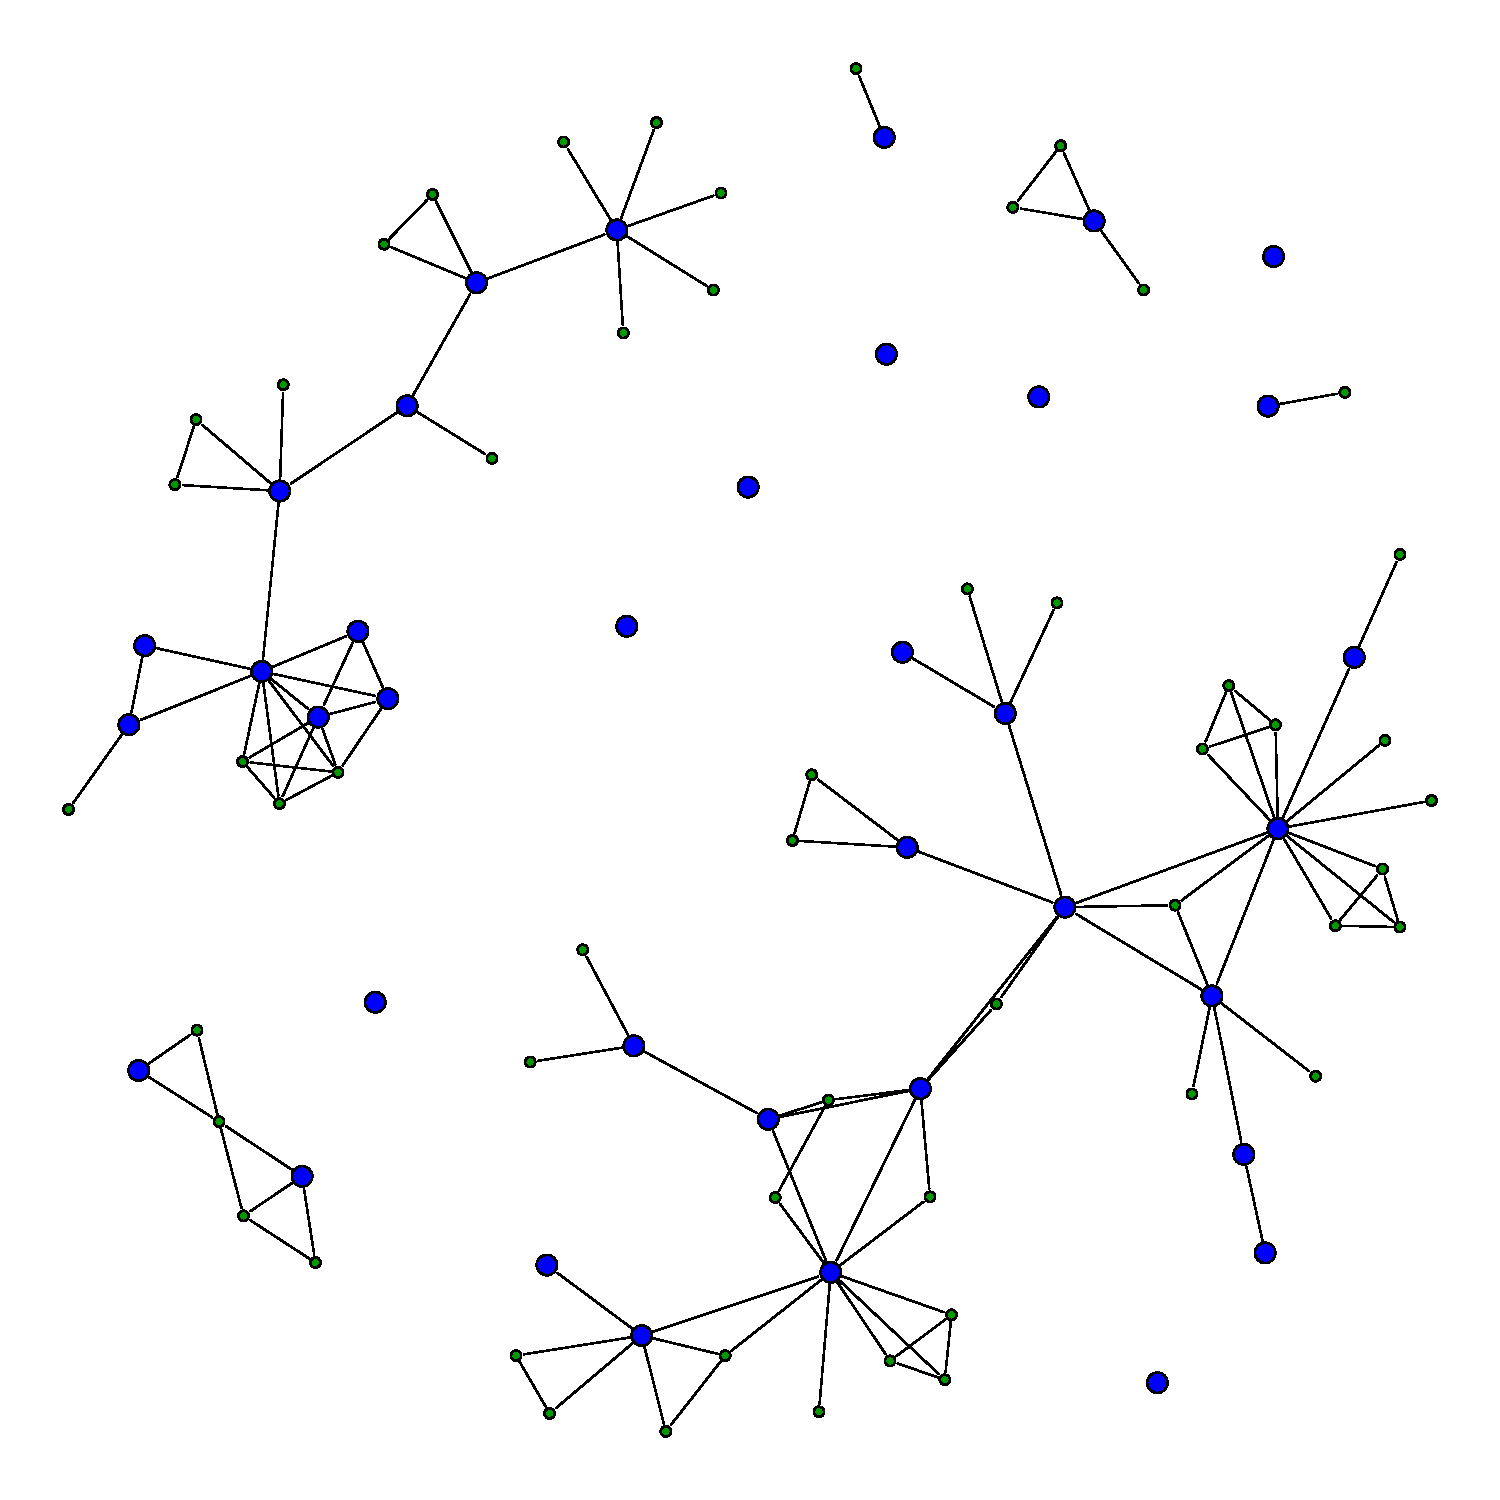
\includegraphics[width=5cm]{figuras/graph}
\caption{\label{fig:graph}Exemplo de uma figura.}
\end{figure}
